%=======================================================================
%  The Cost of Not Being Seen
%  Automated licence-plate reader exposure on American commutes,
%  and the price of avoiding it.
%
%  Build:  tectonic trames.tex
%=======================================================================
\documentclass[11pt,twoside]{article}

\usepackage[T1]{fontenc}
\usepackage[utf8]{inputenc}
\usepackage{lmodern}
\usepackage[margin=1in]{geometry}
\usepackage{graphicx}
\usepackage{booktabs}
\usepackage{amsmath,amssymb}
\usepackage{siunitx}
\usepackage{microtype}
\usepackage{caption}
\usepackage{subcaption}
\usepackage[table]{xcolor}
\usepackage{listings}
\usepackage{enumitem}
\usepackage{authblk}
\usepackage[hidelinks,breaklinks]{hyperref}
\usepackage[capitalise,noabbrev]{cleveref}

\sisetup{group-separator={,},group-minimum-digits=4,detect-weight=true}
\captionsetup{font=small,labelfont=bf,width=.95\linewidth}
\captionsetup[sub]{font=small}
\setlist{itemsep=2pt,parsep=0pt,topsep=3pt}

\definecolor{codebg}{HTML}{F6F6F6}
\lstset{
  basicstyle=\ttfamily\footnotesize,
  backgroundcolor=\color{codebg},
  frame=single, rulecolor=\color{gray!40},
  breaklines=true, showstringspaces=false,
  columns=fullflexible, xleftmargin=0pt, framexleftmargin=3pt,
}

% xspace must be loaded before the macro that uses it is expanded.
\usepackage{xspace}
\usepackage[super]{nth}
\newcommand{\alpr}{ALPR\xspace}

\title{\bfseries The Cost of Not Being Seen:\\[2pt]
\large Automated Licence-Plate Reader Exposure on American Commutes\\
and the Price of Avoiding It}

\author[ ]{TRAMES Project}
\affil[ ]{\small\texttt{kara@soulstone.org}}
\date{\today}

\begin{document}
\maketitle

\begin{abstract}
\noindent
Automated licence-plate readers (\alpr) have moved from tollbooths to residential
intersections, and a single vendor---Flock Safety---now accounts for
\SI{80.0}{\percent} of the \num{142991} installations mapped in North America. Public
argument about this technology is conducted almost entirely in the abstract. We supply a
measurement instead: how much \alpr surveillance a typical American commuter actually
drives through, and what it would cost them to refuse it.

We build a continental routing engine that models \alpr fields of view as directional
geometry---\SI{98.0}{\percent} of mapped cameras carry a bearing---and can be asked for
the fastest route that crosses none of them. Routing \num{17580} real home--work commutes
drawn from Census LEHD LODES data across 15 states, twice each, yields both quantities on
identical road network.

Three findings. First, \SI{78.7}{\percent} of commutes pass at least one \alpr, a median
of three and a \nth{99} percentile of thirty-five. Second, refusal is far cheaper than
expected: \SI{82.1}{\percent} of commutes can be routed to \emph{zero} \alpr exposure for
a median of \SI{1.98}{\minute}, an overhead of \SI{7.90}{\percent}. Third, and most
consequentially for policy, demographic gradients that appear robust nationally---origin
tracts in the highest quartile of Black population pass \num{1.36}$\times$ as many
cameras as the lowest, with disjoint confidence intervals---vanish when tracts are ranked
within their own county ($\num{1.05}\times$, indistinguishable). Mapped camera density
varies \num{3.4}$\times$ per capita across the states we study. We therefore
report the equity result as a between-county phenomenon that this design cannot
attribute to siting, mapping effort, or urban form, and we argue that no study built on
crowdsourced surveillance data should report such a gradient without this check.

Resolving exposure by vendor locates the disparity: tolling and transport-agency cameras
show a gradient of $\num{1.62}\times$ against $\num{1.28}\times$ for Flock, whose
installations are four-fifths of the network. Per unit deployed, non-Flock cameras reach
\num{2.3}$\times$ as many commuters. Flock's gradient dissolves under within-county
ranking; the transport-agency gradient narrows to $\num{1.20}\times$ and remains
distinguishable---the one contrast in the paper that survives the control. Routing the
same commutes against a second snapshot taken two months later, with \SI{18}{\percent}
more mapped cameras, raised measured exposure in exact proportion and left the marginal
price of evading a camera unchanged.

All code, data acquisition, and analysis are reproducible from public sources.
\end{abstract}

\section{Introduction}
\label{sec:intro}

Automated licence-plate readers photograph every passing vehicle, resolve the plate, and
retain the read. Unlike a traffic camera they are not triggered by an offence, and unlike
a patrol officer they do not tire. Fixed, pole-mounted units have spread from limited-access
highways into residential neighbourhoods, arterial roads, and the entrances of private
subdivisions.

The public debate about this expansion is conducted in the vocabulary of policy: retention
windows, warrant requirements, audit logs, data-sharing agreements. What that vocabulary
lacks is a measurement of the thing being regulated. How much of this does a person
actually drive through on an ordinary Tuesday? And if they would rather not, is declining
a practical option or a theoretical one?

This paper answers both, and does so by building the instrument the question implies. We
construct a routing engine that treats \alpr fields of view as first-class geometry and
can be asked for the fastest route that avoids them. Running each sampled commute through
it twice---once normally, once avoiding---yields the exposure and the price of refusing
it, for the same trip, on the same network, under the same traffic model.

The second quantity is where the paper earns its keep. A privacy protection that costs
four minutes is a feature. One that costs forty is available only to people with forty
minutes to spare, and a right that is priced is not evenly held. We therefore report the
cost of refusal across origin-tract income and racial composition---subject to the
substantial caveat developed in \Cref{sec:coverage} and quantified in
\Cref{sec:results:coverage}, which turns out to govern how the demographic results may be
read.

\subsection{Contributions}

\begin{itemize}
  \item \textbf{A directional exposure model at continental scale.} Cameras are wedges,
    not circles. \SI{98.0}{\percent} of mapped North American \alpr installations carry a
    bearing tag, making this feasible nationally. Proximity-based counting inflates
    exposure by charging drivers for cameras aimed at the opposite carriageway; we do not
    do it.
  \item \textbf{Avoidance routing with no forked router.} \num{135210} camera cones are
    compiled into a stock GraphHopper spatial index at import time, so an ordinary
    per-request custom model can reference them by name. No engine patches, no geometry in
    the request.
  \item \textbf{A commute-weighted rather than area-weighted sample.} \num{17580} real
    home--work pairs drawn from LEHD LODES with probability proportional to worker count.
  \item \textbf{A vendor-resolved account of exposure.} Flock and the DOT/tolling vendors
    follow different deployment logics---who \emph{buys} surveillance versus where road
    infrastructure sits. Separating them shows the national racial gradient is
    substantially stronger in transport infrastructure than in the vendor that dominates
    both the network and the public argument about it.
  \item \textbf{A coverage-bias control that changes the conclusion.} We show that the
    national demographic gradient does not survive within-county ranking, quantify the
    \num{3.4}$\times$ per-capita spread in mapping intensity that plausibly drives it, and
    argue this check should be mandatory for work of this kind.
  \item \textbf{A paired re-measurement.} The same commutes routed against a snapshot
    taken two months later with \SI{18}{\percent} more mapped cameras: exposure rose in
    proportion, the marginal price of evading a camera did not move, and the states we had
    flagged as under-mapped are the ones that grew most.
\end{itemize}

\section{System}
\label{sec:system}

\subsection{Why a fork, and of what}

The measurement needs a router that treats ``avoid these \num{135210} polygons'' as a
cost rather than a post-hoc filter, and the eventual application needs to be a real
navigation client rather than a research script.

\textbf{OsmAnd} (GPLv3) is the base: the only mature Android navigation client with
first-class OpenStreetMap support, offline maps, and a documented online-routing extension
point. Its \emph{code} is GPLv3; its \emph{artwork} is CC-BY-NC-ND 4.0 and must therefore
be replaced rather than modified in a derivative.

\textbf{GraphHopper 11.0} is the routing engine. Valhalla was evaluated and rejected: its
\texttt{exclude\_polygons} support carries open correctness defects (\#3266, \#4659,
\#5069) whose failure mode is silently routing \emph{through} the excluded region---which
is precisely the measurement everything here depends on.

One architectural property made the rest tractable. OsmAnd's online routing engines return
\emph{geometry only}; turn instructions are re-derived client-side from offline map data.
A custom online router therefore never has to synthesise navigation instructions.

\subsection{The keystone: import-time custom areas}

GraphHopper resolves \texttt{custom\_areas.directory} into a spatial index \emph{at graph
import time}. We verified empirically---the documentation is ambiguous---that an area
registered this way can be referenced by name from a \emph{per-request} custom model:

\begin{lstlisting}[language=]
{ "priority": [ { "if": "in_alpr", "multiply_by": 0.01 } ] }
\end{lstlisting}

\noindent
This is what makes the design possible without forking the engine; shipping \num{135210}
polygons in every routing request is not viable. The cost is that regenerating cones
requires a full re-import (\SI{82}{\minute} to \SI{113}{\minute} for North America, by load).

Two further configuration decisions are load-bearing:

\begin{itemize}
  \item \textbf{Contraction Hierarchies are disabled.} CH bakes edge weights into the
    prepared graph, which is incompatible with a per-request avoidance strength. Landmarks
    (LM) are used instead.
  \item \textbf{The \texttt{car\_alpr} profile shares \texttt{car}'s LM preparation.} This
    halves preparation time and is valid \emph{only} because avoidance multiplies priority
    strictly downward, so the borrowing profile's weights never exceed the preparation
    profile's on any edge---the condition LM correctness requires.
\end{itemize}

\subsection{Deployment posture}

The routing server binds to localhost. It has no authentication and no rate limiting and
is not internet-facing. Any public deployment must sit behind a reverse proxy supplying
both.

\section{Data}
\label{sec:data}

All sources are public and key-free.

\subsection{ALPR installations}
\label{sec:data:alpr}

Source: OpenStreetMap via the Overpass API, selecting
\texttt{man\_made=surveillance} with \texttt{surveillance:type=ALPR}, matched
case-insensitively (19 readers are tagged \texttt{alpr})---the corpus surfaced by the
DeFlock project, taken from the upstream rather than a mirror. Retrieved in five regional
queries (continental US, Alaska, Hawaii, Canada, Mexico) and deduplicated by OSM node id.
The results in this paper rest on the snapshot of \textbf{2026-09-22: \num{142991} unique
camera nodes} (\Cref{fig:map}). A first snapshot, taken 2026-07-24, held \num{120838};
\Cref{sec:results:refresh} routes the same commutes against both.

A fetch that fails over between Overpass mirrors has to check the mirror's database
date. On the first attempt at the September snapshot one regional query fell through to
a mirror whose database was dated 2026-05-06; that box overlaps the southern United
States, regions were merged last-wins, and roughly \num{13600} cameras across Texas,
Arizona and Florida silently reverted to four-month-old tags while some \num{400} nodes
deleted since May returned as ghosts. Nothing failed. The fetch now rejects any answer
older than 48 hours and merges overlapping regions newest-database-first; every tile of
the snapshot used here falls within a 13-minute window.

\begin{table}[t]
\centering
\small
\caption{Directional and vendor tagging across the two snapshots. The direction-key rows
overlap (392 and 415 nodes carry both keys). Vendors are matched as case-insensitive
substrings under any of the four vendor keys, in both columns.}
\label{tab:tags}
\begin{tabular}{lrrrr}
\toprule
& \multicolumn{2}{c}{2026-07-24} & \multicolumn{2}{c}{2026-09-22} \\
\cmidrule(lr){2-3}\cmidrule(lr){4-5}
Property & Count & Share & Count & Share \\
\midrule
Camera nodes                        & \num{120838} &                     & \num{142991} & \\
Any direction tag                   & \num{119249} & \SI{98.7}{\percent} & \num{140112} & \SI{98.0}{\percent} \\
\quad via \texttt{direction}        & \num{117356} & \SI{97.1}{\percent} & \num{138216} & \SI{96.7}{\percent} \\
\quad via \texttt{camera:direction} & \num{2285}   & \SI{1.9}{\percent}  & \num{2311}   & \SI{1.6}{\percent} \\
Multi-head (\texttt{;}-separated)   & \num{7014}   & \SI{5.8}{\percent}  & \num{9150}   & \SI{6.4}{\percent} \\
Arc-range form (\texttt{199-269})   & \num{4806}\,tokens & ---           & \num{4632}\,tokens & --- \\
\texttt{operator} tagged            & \num{22354}  & \SI{18.5}{\percent} & \num{23872}  & \SI{16.7}{\percent} \\
\midrule
Flock Safety                        & \num{99650}  & \SI{82.5}{\percent} & \num{114360} & \SI{80.0}{\percent} \\
Motorola Solutions                  & \num{5993}   & \SI{5.0}{\percent}  & \num{7411}   & \SI{5.2}{\percent} \\
Genetec                             & \num{2876}   & \SI{2.4}{\percent}  & \num{3721}   & \SI{2.6}{\percent} \\
Leonardo                            & \num{1020}   & \SI{0.8}{\percent}  & \num{1215}   & \SI{0.8}{\percent} \\
Axis Communications                 & \num{1052}   & \SI{0.9}{\percent}  & \num{3327}   & \SI{2.3}{\percent} \\
No vendor tag                       & \num{5811}   & \SI{4.8}{\percent}  & \num{6850}   & \SI{4.8}{\percent} \\
\bottomrule
\end{tabular}
\end{table}

Three tagging realities shaped the parser, each contradicting a plausible assumption:

\begin{enumerate}
  \item \textbf{\texttt{direction}, not \texttt{camera:direction}.} The OSM wiki documents
    \texttt{camera:direction} for surveillance nodes. Mappers overwhelmingly use plain
    \texttt{direction}, by a factor of 60. Reading only the documented key discards
    \SI{97}{\percent} of the bearings.
  \item \textbf{Arc ranges are real, and mostly \ang{45}.} \num{4632} values give an
    explicit range; \num{3806} of them (\SI{82}{\percent}) span exactly \ang{45}. That is
    what justifies \ang{45} as the default span for the \(\approx\)\SI{97}{\percent} of
    cameras giving a bare bearing---the default is inherited from the data, not assumed.
  \item \textbf{Multi-head units exist} (\texttt{320;190},
    \texttt{0;72;144;216;288}, \texttt{199-269;325-35}); \num{9150} nodes. These typically
    watch \emph{both} carriageways, so silently taking the first bearing is the worst
    available error: it makes a camera that sees everyone look like one that sees half.
    The parser emits one wedge per head.
\end{enumerate}

\begin{figure}[t]
\centering
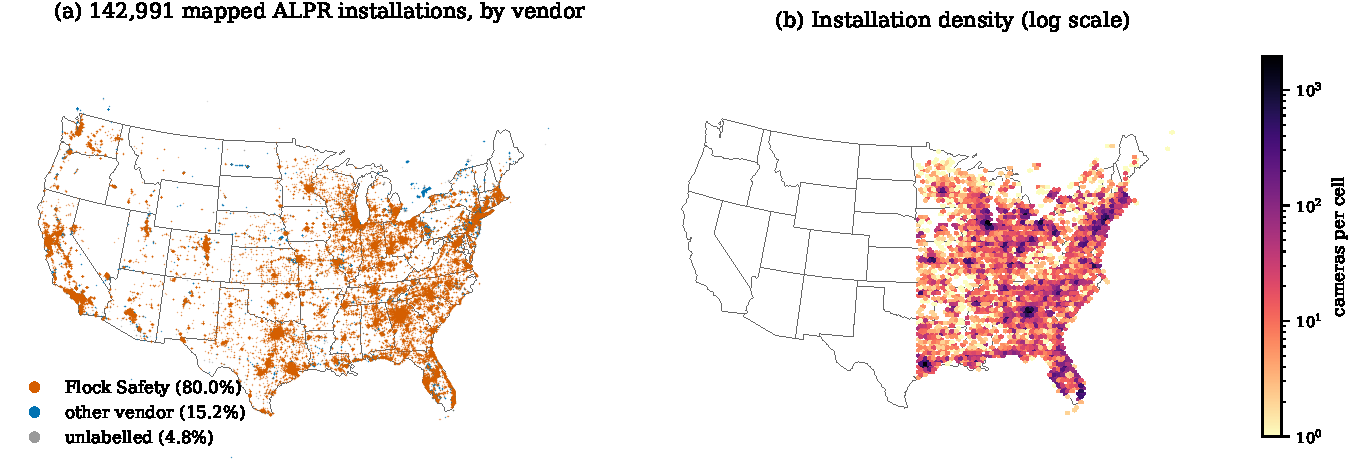
\includegraphics[width=\linewidth]{figures/fig_camera_map.pdf}
\caption{Mapped \alpr installations in the contiguous United States. (a) By vendor: Flock
Safety dominates by count almost everywhere, with other vendors concentrated on
limited-access corridors. (b) Density on a log scale. The visible structure is partly
deployment and partly \emph{mapping}: see \Cref{sec:results:coverage}.}
\label{fig:map}
\end{figure}

\subsection{Cone construction}
\label{sec:data:cones}

Each camera head becomes a circular sector: apex at the node, bisector along the tagged
bearing, span \ang{45} (or the tagged arc), radius \SI{60}{\metre}. The radius must reach
across the carriageway from a set-back pole; it was chosen on that reasoning and then swept
over $\{30,45,60,90\}\,\si{\metre}$ (\Cref{sec:lim:geom}). Measured exposure is only mildly
sensitive to it, but the avoidance result is not robust above the assumed value.

All wedges are unioned into a single MultiPolygon of \textbf{\num{135210} parts},
published as one feature with id \texttt{alpr}. Overlapping wedges merging is correct and
intended: the question is \emph{is this road segment observed}, not \emph{by how many
devices}.

\begin{table}[t]
\centering
\small
\caption{Vendor-split cone sets, 2026-09-22 snapshot. The cones-per-camera column is
itself a result: non-Flock installations are multi-head more than six times as often
(\SI{22.8}{\percent} against \SI{3.6}{\percent}), consistent with tolling and DOT gantries
covering every lane while a Flock unit watches one approach.}
\label{tab:vendorsets}
\begin{tabular}{lrrrr}
\toprule
Set & Cameras & Cones & Cones/camera & Union parts \\
\midrule
Flock Safety       & \num{113611} & \num{120366} & 1.06 & \num{109427} \\
Other named vendor & \num{20435}  & \num{30128}  & \textbf{1.47} & \num{21587} \\
No vendor tag      & \num{5997}   & \num{6590}   & 1.10 & \num{5211} \\
\bottomrule
\end{tabular}
\end{table}

Assigning vendor requires care. Vendor appears under four keys
(\texttt{manufacturer}, \texttt{surveillance:manufacturer}, \texttt{brand},
\texttt{surveillance:brand}) and is spelled inconsistently. An exact match on
\texttt{manufacturer = "Flock Safety"} finds \num{109892} cameras; a case-insensitive
substring search across all four finds \num{114360}. The \num{4468} difference is mostly
\num{4711} nodes carrying the vendor under \texttt{brand}, plus variants (``Flock Group
Inc.'', ``FlockSafety''). Misfiling \SI{3.9}{\percent} of Flock cameras as non-Flock is
the one error a vendor comparison cannot absorb.

Untagged cameras are held out of \emph{both} vendor sets rather than assigned to the
complement of Flock, since an untagged camera is likelier to be an unlabelled Flock unit
than a non-Flock one. They are reported as their own set so nothing is silently dropped,
with the caveat that their direction coverage is lower (\SI{88.0}{\percent} against
\SI{99.4}{\percent} for Flock and \SI{93.8}{\percent} for other named vendors---the last
down from \SI{98.5}{\percent} in July, as newly mapped Axis units often arrive without a
bearing).

\subsection{Road network}

Geofabrik North America extract, \SI{18}{\giga\byte}, retrieved 2026-07-24 and held
fixed for both snapshots, so that \Cref{sec:results:refresh} isolates the camera data:
every unavoided route is identical between the two runs to the metre. Imported with
\texttt{ignored\_highways = footway,construction,cycleway,path,steps}. \texttt{track} is
deliberately retained: unpaved tracks are plausible avoidance routes, and excluding them
would bias the cost estimate downward by removing options a determined driver has.

\subsection{Commute sample}
\label{sec:data:commutes}

Source: LEHD \textbf{LODES8}, \texttt{od\_main\_JT00}, 2022---all jobs, both ends
in-state, built from unemployment-insurance wage records linked to employer
establishments. These are administrative counts of real jobs, not survey estimates.

Sampling design carries more weight here than sample size. Uniform random points would
over-represent empty rural space where nobody commutes and no cameras exist, understating
exposure badly. Instead each origin--destination pair is drawn \textbf{with probability
proportional to the number of workers actually making that trip}, so the distribution
approximates what an average \emph{commuter} experiences rather than what an average
\emph{square kilometre} contains.

Block-level LODES geocodes are aggregated to \textbf{tract} (first 11 digits)---the finest
resolution at which ACS demographics are reliable, and finer than the routing's effective
precision. Same-tract commutes are dropped: origin and destination centroids coincide, so
there is no route to measure. Georgia alone yields \num{1199250} distinct tract pairs
covering \num{4190313} workers.

\num{1200} pairs are requested per state; duplicate draws are collapsed, costing
\SI{0.53}{\percent}, for \textbf{\num{17904} sampled commutes} across 15 states (AZ, CA,
CO, FL, GA, IL, MO, NC, NY, OH, PA, TN, TX, VA, WA). Seed \texttt{20260725}; the sample is
reproducible. The sampled pairs represent \num{600899} workers; the median pair carries 10
and the largest \num{2832}.

Because draws are taken with replacement and then deduplicated, each pair appears once and
every row is weighted equally downstream. That is valid only while inclusion probability
remains proportional to worker count, which decays once a pair is likely to be drawn more
than once. Measured on Georgia, the largest state sample, the highest-flow pair has an
expected \num{0.22} draws per \num{1200} and a median pair \num{0.0036}: the design is
probability-proportional-to-size with distortion confined to the extreme upper tail
(roughly \SI{11}{\percent} under-representation for the single largest pair, negligible
below it). The \texttt{workers} and \texttt{flow\_share} columns are carried through the
pipeline but deliberately unused---equal weighting already yields the worker-weighted
distribution, and weighting again would apply the flow twice.

\subsection{Demographics and geography}

Tract centroids are 2024 Census Gazetteer internal points
(\texttt{INTPTLAT}/\texttt{INTPTLONG}), which are guaranteed to fall inside the tract
polygon. Income is ACS 5-year 2022 table \textbf{B19013}; race and ethnicity are table
\textbf{B03002}, chosen over B02001 because it is Hispanic-aware, so ``non-Hispanic
Black'' is directly available rather than reconstructed. Demographics attach to the
\emph{origin} (home) tract: the claim under test concerns who lives where surveillance is
dense.

\section{Method}
\label{sec:method}

\subsection{Two routes per commute}

Each sampled pair is routed twice against the same graph: a \textbf{baseline} with no
custom model, and an \textbf{avoided} route applying
\texttt{priority: [\{if: "in\_alpr", multiply\_by: 0.01\}]}. Both disable CH, which
per-request custom models require.

\num{0.01} is the \emph{maximum} avoidance strength, not a typical setting. Results
therefore describe an \textbf{upper bound on both the benefit and the cost} of
avoidance---the strongest available preference short of prohibition. This is deliberate:
it establishes whether meaningful avoidance is possible at all, and what it costs at the
limit.

\subsection{Exposure is directional, not proximate}

A camera counts as having seen the driver \emph{only if the route line intersects its
cone}. Passing \SI{20}{\metre} from a camera aimed the other way is not exposure.
Implementation is an STRtree over the \num{135210} cone parts for candidate lookup, then
an exact intersection test.

Two conservatisms remain, both understating exposure: route geometry is a polyline while a
vehicle has width, and a cone occluded by intervening buildings is still counted as full
sight-line.

\subsection{Vendor attribution costs no additional routing}

Routing does not change between vendor questions---the avoidance model targets the
all-vendor union either way---so \Cref{sec:results:vendor} is entirely a matter of
re-scoring existing routes against different cone sets. This is possible only because the
experiment persists route polylines to a sidecar; keeping only counts would have made both
the vendor split and the radius sweep of \Cref{sec:lim:geom} fresh multi-hour re-runs.

As a consistency check, the three vendor sets should sum to slightly \emph{more} than the
all-vendor union, because cones from different vendors that overlap merge into one part in
the union and are counted once while the split sets count them separately. Measured excess
is \SI{1.0}{\percent}: right sign, plausible magnitude.

\subsection{Statistical reporting}
\label{sec:method:stats}

\begin{itemize}
  \item \textbf{Medians lead, means accompany.} Both distributions are heavily
    right-skewed; a minority of long commutes through dense corridors pull the mean well
    above the typical experience.
  \item \textbf{Bootstrap confidence intervals} (percentile, \num{2000} resamples, seed
    \texttt{20260725}). Camera counts are discrete and zero-inflated, nowhere near normal.
  \item \textbf{Quartile contrasts, not regressions.} With tract-level aggregates a
    regression coefficient invites a causal reading the design cannot support.
  \item \textbf{Total exposure and per-kilometre density are reported as peers.} A raw
    count gap that vanishes once normalised per km is about distance, not siting. But the
    converse is a finding, not a nuisance: a group whose commutes are \emph{shorter but
    more densely watched} shows a rate gap and no count gap, and treating the rate purely
    as a control would discard it. Cameras per km is a ratio of sums bootstrapped over
    commutes; a mean of per-commute rates would let very short commutes dominate.
  \item \textbf{Ecological inference is not attempted.} Tract composition is a property of
    tracts, not of the individuals routed.
\end{itemize}

\subsection{Execution}
\label{sec:method:exec}

Twelve concurrent workers against the local routing server. Worker count was measured, not
assumed: twelve completed 300 commutes in \SI{324}{\second}, while thirty-two took longer
than \SI{576}{\second} on the identical set---past about twelve, contention outweighs added
concurrency. Routing dominates cost overwhelmingly; the geometric exposure test is
\SI{0.2}{\percent} of per-commute work.

Failed routes are dropped rather than retried: failures are dominated by unroutable
centroid pairs (islands, centroids landing off-network), properties of the sample rather
than transient faults. \textbf{\num{17580} of \num{17904} commutes routed successfully
(\SI{1.8}{\percent} dropped)}---the same \num{324} failures in both snapshots. The
September run took \SI{10.6}{\hour} against \SI{5.4}{\hour} for July on the same
hardware: with a fifth more penalised edges, the avoiding search visits more of the graph.

Commutes are processed in seeded random order. The sample is grouped by state and the
executor preserves input order, so in file order results arrive one state at a time: an
interruption would leave some states complete and others absent, and no partial output
could support a national estimate. Shuffling makes any prefix a near-uniform sample of the
whole. This proved material rather than hypothetical---an earlier single-state interim
read gave a median avoidance overhead of \SI{22.7}{\percent} against that run's national
\SI{5.96}{\percent}.

\section{Results}
\label{sec:results}

\subsection{Exposure on the unavoided commute}
\label{sec:results:exposure}

\begin{table}[t]
\centering
\small
\caption{Exposure and the cost of avoidance over \num{17580} commute-weighted
origin--destination pairs in 15 states. Median commute \SI{24.4}{\kilo\metre} /
\SI{24.1}{\minute}.}
\label{tab:headline}
\begin{tabular}{lrr}
\toprule
& Median [\SI{95}{\percent} CI] & Mean \\
\midrule
\multicolumn{3}{l}{\itshape Unavoided route} \\
Cameras passed              & 3 [3--3]            & 5.63 \\
Commutes passing $\geq$1    & \multicolumn{2}{r}{\SI{78.7}{\percent}} \\
Commutes passing $\geq$5    & \multicolumn{2}{r}{\SI{39.7}{\percent}} \\
Commutes passing $\geq$10   & \multicolumn{2}{r}{\SI{18.3}{\percent}} \\
\nth{90} / \nth{99} percentile & \multicolumn{2}{r}{14 / 35 cameras} \\
Exposure rate               & \multicolumn{2}{r}{\num{0.105} cameras/\si{\kilo\metre}} \\
\midrule
\multicolumn{3}{l}{\itshape ALPR-avoiding route} \\
Cameras passed              & 0 [0--0]            & 0.30 \\
\textbf{Reduced to zero}    & \multicolumn{2}{r}{\textbf{\SI{82.1}{\percent}}} \\
Extra time (\si{\minute})   & \textbf{1.98} [1.89--2.07] & 5.97 \\
Extra distance (\si{\kilo\metre}) & 0.76 [0.72--0.79] & 2.69 \\
Avoidance overhead          & \SI{7.90}{\percent} [7.60--8.17] & \SI{14.22}{\percent} \\
Minutes per camera evaded   & 0.78 [0.77--0.80]   & 1.31 \\
\bottomrule
\end{tabular}
\end{table}

\begin{figure}[t]
\centering
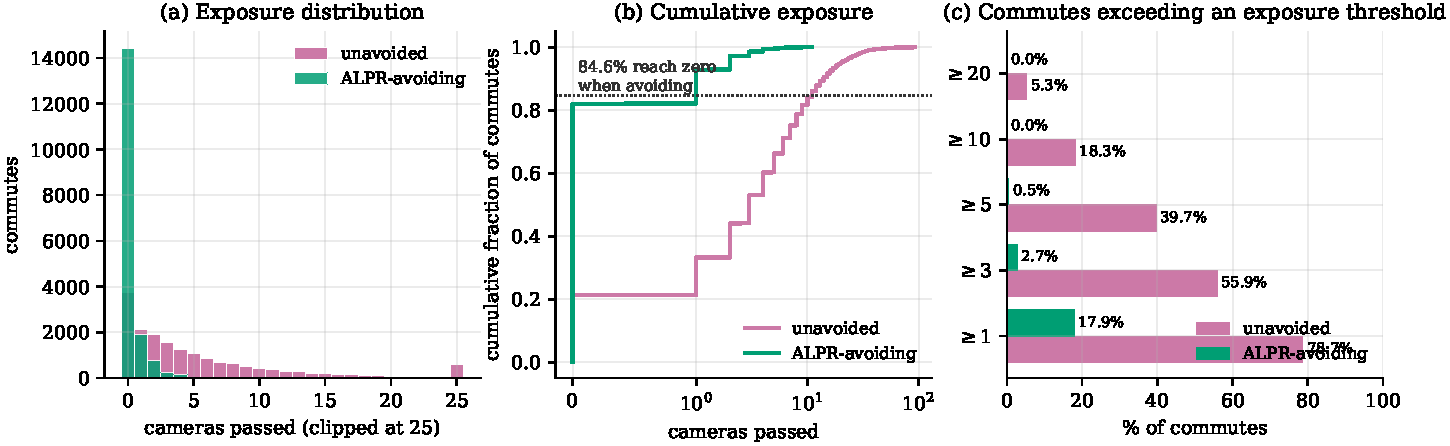
\includegraphics[width=\linewidth]{figures/fig_exposure.pdf}
\caption{Exposure before and after \alpr-avoiding routing. (a) Distributions; (b)
cumulative, log-scaled abscissa; (c) share of commutes exceeding a threshold. The
zero-exposure mass moves from \SI{21.3}{\percent} to \SI{82.1}{\percent}.}
\label{fig:exposure}
\end{figure}

\textbf{\SI{78.7}{\percent} of American commutes pass at least one \alpr.} The median
commuter is read three times each way; the \nth{90} percentile fourteen times and the
\nth{99} thirty-five. Aggregate exposure is \num{0.105} cameras per kilometre driven.

\subsection{The cost of refusal}
\label{sec:results:cost}

\begin{figure}[t]
\centering
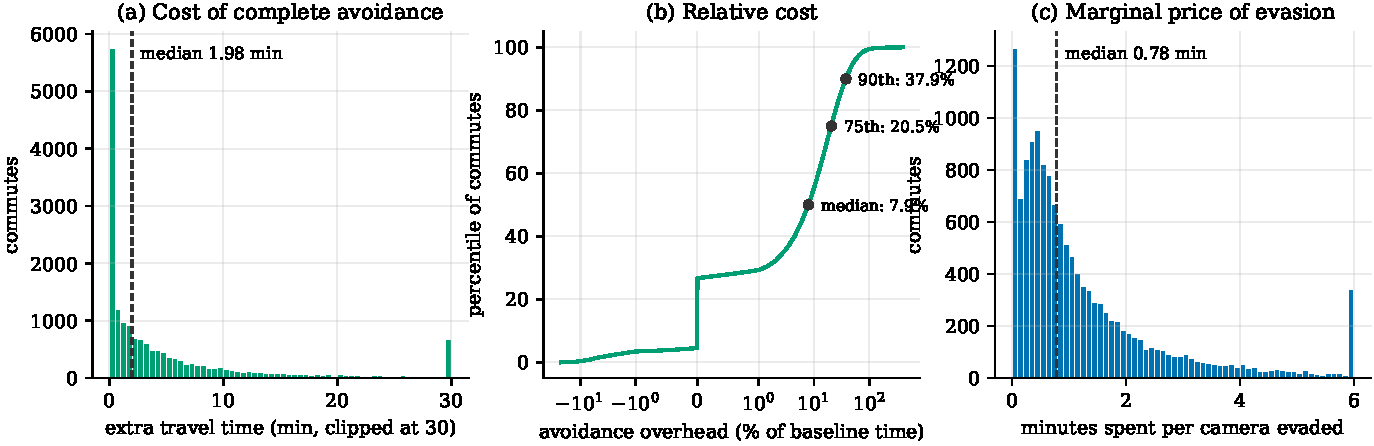
\includegraphics[width=\linewidth]{figures/fig_cost.pdf}
\caption{The price of complete avoidance. (a) Absolute extra time; (b) overhead as a
percentage of baseline, by percentile; (c) marginal minutes per camera evaded. All three
are heavily right-skewed---a small tail of commutes pays a great deal, while the typical
commute pays almost nothing.}
\label{fig:cost}
\end{figure}

\textbf{\SI{82.1}{\percent} of commutes can be routed to zero \alpr exposure}, at a median
cost of \SI{1.98}{\minute} and \SI{0.76}{\kilo\metre}---an overhead of
\SI{7.90}{\percent}. The median marginal price is \SI{0.78}{\minute} per camera evaded.

For four American commuters in five, then, complete avoidance of licence-plate
surveillance costs about two minutes. This figure is conditional on the assumed camera
field of view: it is stable if the true radius is smaller than the \SI{60}{\metre} assumed
here and degrades if it is substantially larger, which \Cref{sec:lim:geom} quantifies. This is the paper's central quantitative claim,
and it is considerably more favourable than the metropolitan spot-checks that motivated
the study suggested.

The distribution matters as much as the median. The mean overhead is \SI{14.22}{\percent}
against a median of \SI{7.90}{\percent}, and the interquartile range runs from
\SI{0}{\percent} to \SI{20.6}{\percent}: a quarter of commutes need no detour whatsoever,
while a tail pays substantially. \Cref{fig:route} shows one such case.

\begin{figure}[t]
\centering
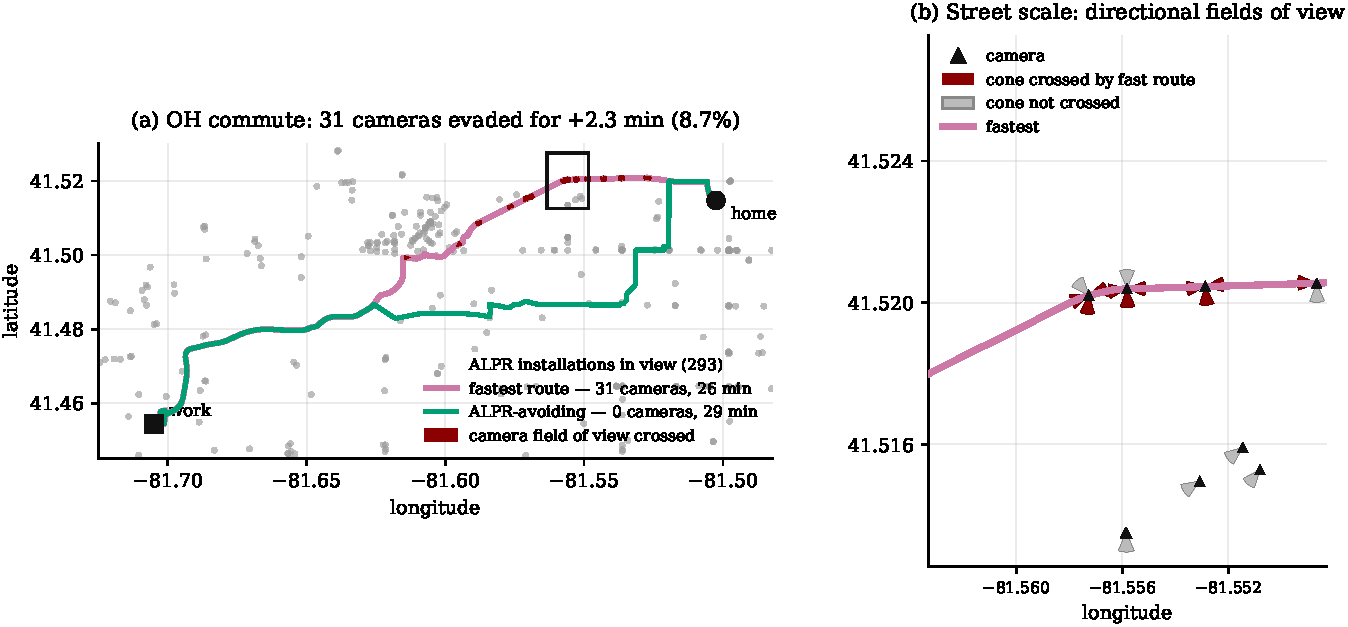
\includegraphics[width=\linewidth]{figures/fig_route_example.pdf}
\caption{An illustrative high-exposure commute in the Cleveland area---chosen for
legibility, not typicality. (a) The fastest route crosses 31 camera fields of view; the
avoiding route crosses none, for \SI{+2.3}{\minute} (\SI{8.7}{\percent}). (b) At street scale the
directional model is visible: cones the fast route crosses are dark, cones aimed elsewhere
are grey and cost nothing.}
\label{fig:route}
\end{figure}

\subsection{Geographic variation}
\label{sec:results:geo}

\begin{figure}[t]
\centering
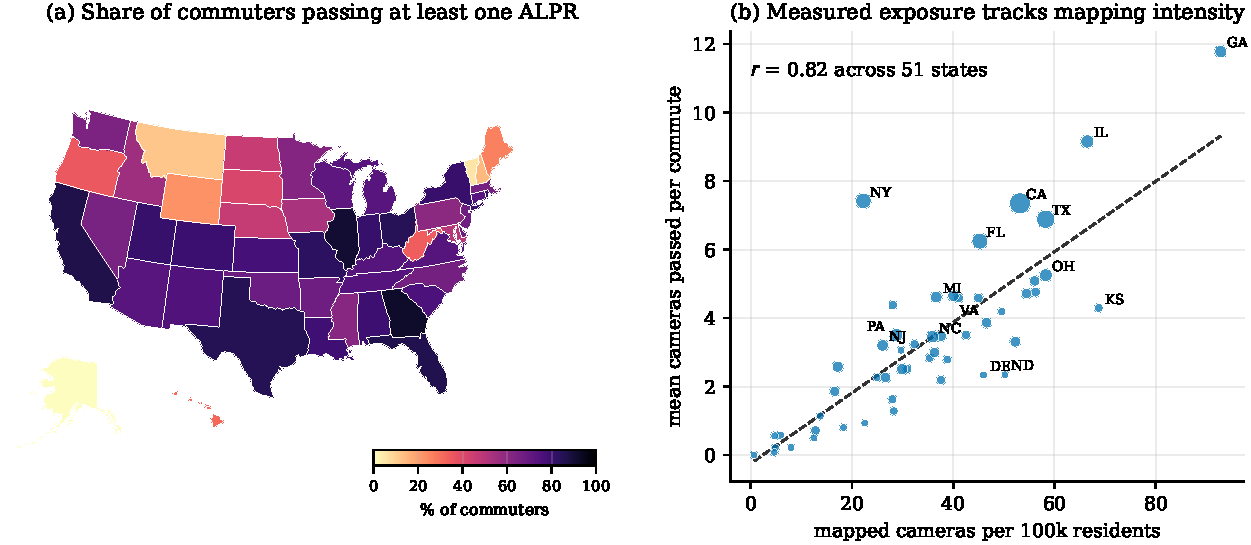
\includegraphics[width=\linewidth]{figures/fig_states.pdf}
\caption{(a) Mean exposure by state with median avoidance overhead overlaid. (b) State
exposure against mapped cameras per \num{100000} residents. The relationship is close to
linear, which is the central interpretive problem of \Cref{sec:results:coverage}: we
cannot separate ``more cameras'' from ``more mappers''.}
\label{fig:states}
\end{figure}

State-level variation is extreme. Georgia commuters pass a median of eight cameras and pay
\SI{25.8}{\percent} overhead to avoid them; Pennsylvania commuters pass a median of one
and pay \SI{1.3}{\percent}, with \SI{60}{\percent} passing any camera at all---up from
\SI{41}{\percent} two months earlier (\Cref{sec:results:refresh}).

A robust secondary finding: \textbf{avoidance is cheapest where cameras are densest}.
Dense metropolitan grids offer a parallel street one block over, so the detour is short;
rural and intercity routes often have one viable road, so avoidance means a genuine
detour. The burden of refusal therefore falls hardest on drivers who have the fewest
cameras to refuse---the reverse of the natural guess.

\subsection{Demographic contrasts}
\label{sec:results:demo}

\begin{figure}[t]
\centering
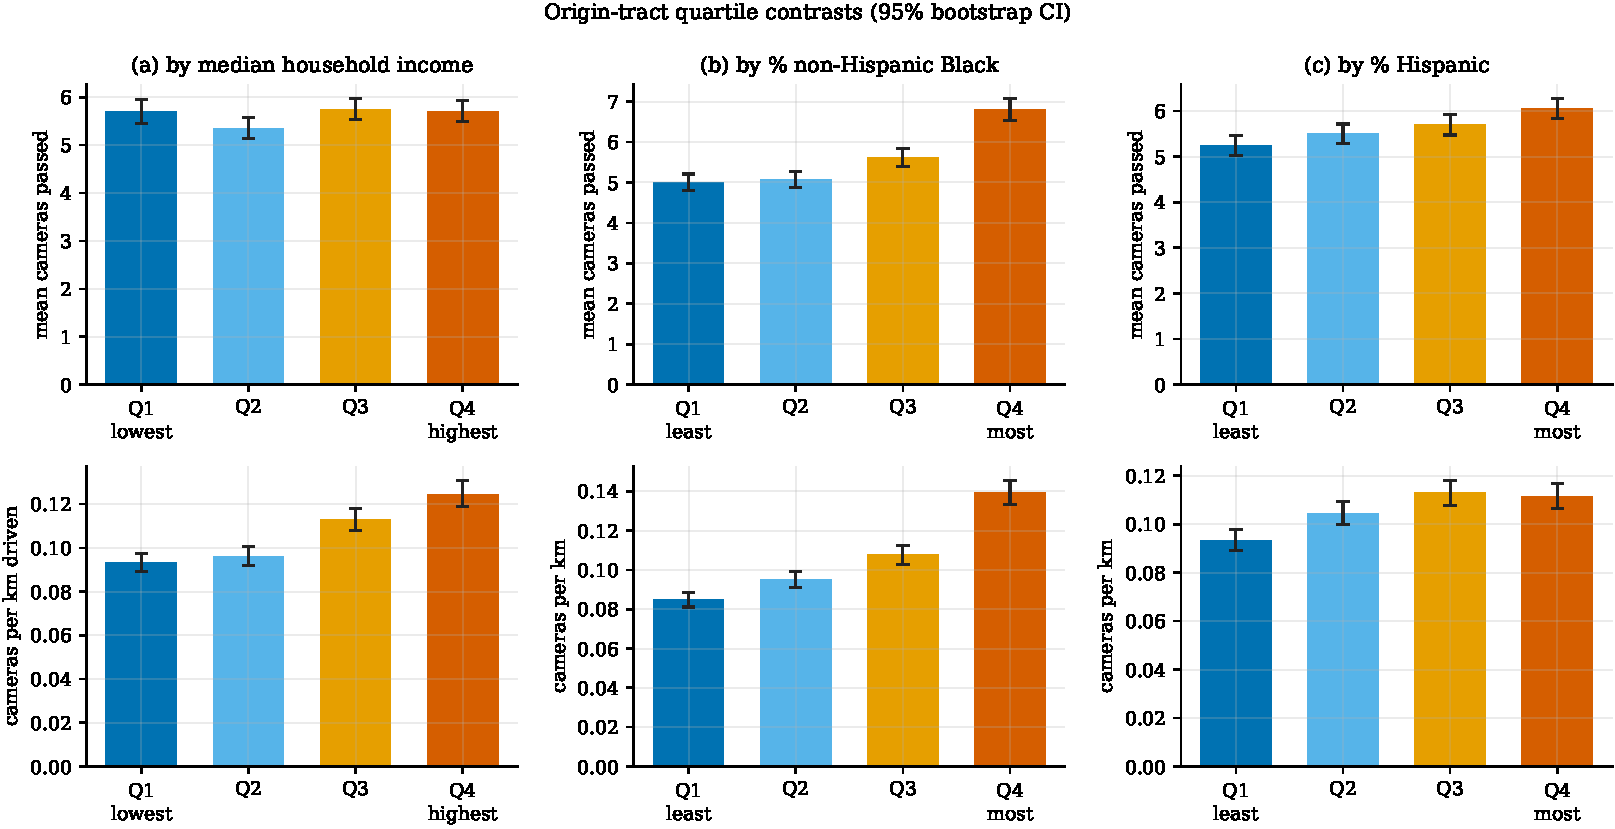
\includegraphics[width=\linewidth]{figures/fig_demographics.pdf}
\caption{Origin-tract quartile contrasts, \SI{95}{\percent} bootstrap CIs. Top row: mean
cameras passed. Bottom row: cameras per kilometre driven. Income shows a per-km gradient
with no count gradient---higher-income origins have denser but shorter commutes.}
\label{fig:demo}
\end{figure}

\begin{table}[t]
\centering
\small
\caption{National quartile contrasts. ``Disjoint'' marks non-overlapping
\SI{95}{\percent} bootstrap CIs.}
\label{tab:demo}
\begin{tabular}{lrrl}
\toprule
Contrast & Ratio & Cameras/\si{\kilo\metre} (Q1 vs Q4) & Verdict \\
\midrule
Income Q1/Q4          & 1.00 & \num{0.0933} vs \num{0.1246} & count overlaps; rate disjoint \\
\% non-Hisp.\ Black Q4/Q1 & \textbf{1.36} & \num{0.0848} vs \num{0.1393} & both disjoint \\
\% Hispanic Q4/Q1     & \textbf{1.15} & \num{0.0933} vs \num{0.1116} & both disjoint \\
\bottomrule
\end{tabular}
\end{table}

Both racial contrasts are statistically distinguishable nationally. Income is not, in
counts---but higher-income origin tracts show materially \emph{denser} per-kilometre
exposure (\num{0.1246} against \num{0.0933}) offset by shorter commutes. Only reporting
count and rate as peers surfaces that; a design treating the rate as a mere control would
have discarded it.

\subsection{Coverage-bias sensitivity, and why it governs the reading}
\label{sec:results:coverage}

\begin{figure}[t]
\centering
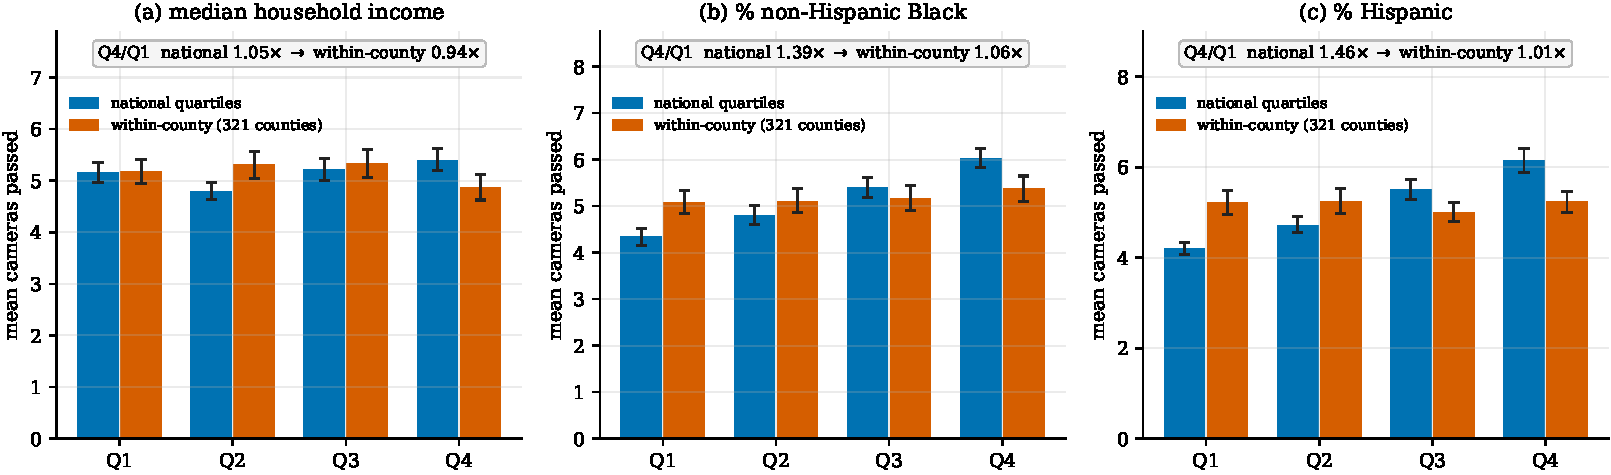
\includegraphics[width=\linewidth]{figures/fig_within_county.pdf}
\caption{The central negative result. Ranking origin tracts within their own county rather
than nationally collapses both demographic gradients to indistinguishability. \num{100}
counties with $n\geq40$ contribute \SI{60}{\percent} of the sample.}
\label{fig:within}
\end{figure}

\Cref{fig:within} is the most consequential figure in the paper. Recomputing quartiles
\emph{within each county} and pooling---so tracts are ranked only against neighbours
subject to the same local mapping effort and broadly the same urban form---collapses the
racial gradient from \num{1.36}$\times$ (disjoint CIs) to \num{1.05}$\times$
(indistinguishable), and leaves income at \num{0.92}$\times$ (indistinguishable).
Within-county per-kilometre rates are close: \num{0.1311} against \num{0.1423}.

The demographic gradients are therefore \textbf{entirely a between-county phenomenon}.

Mapped camera density varies enormously across the states studied---from roughly 108 per
\num{100000} residents in Georgia to 32 in Washington, a \textbf{\num{3.4}$\times$
spread} (\num{3.9}$\times$ in July, before Pennsylvania's mapped density rose by
half)---and state mean exposure tracks it closely (\Cref{fig:states}b). From one snapshot
we cannot distinguish ``Pennsylvania has few cameras'' from ``Pennsylvania has few
mappers''; \Cref{sec:results:refresh} shows what two snapshots can say.

Three explanations remain consistent with these data, and this design separates none of
them:
\begin{enumerate}
  \item \textbf{Differential mapping effort.} Volunteer contributors are unevenly
    distributed, and where they are absent cameras are absent from the map but present on
    the pole.
  \item \textbf{Urban form.} High-\%Black tracts are disproportionately urban and urban
    roads carry more cameras per kilometre, so the national contrast is substantially an
    urban/rural contrast.
  \item \textbf{Genuine between-jurisdiction procurement differences.} Municipalities
    really do differ in what they buy.
\end{enumerate}

We therefore decline to report a national demographic finding as a finding about
surveillance siting. What we report is narrower and defensible: a gradient exists in the
observable data, it is between-county, and it does not survive local ranking.

\subsection{By camera vendor}
\label{sec:results:vendor}

\begin{figure}[t]
\centering
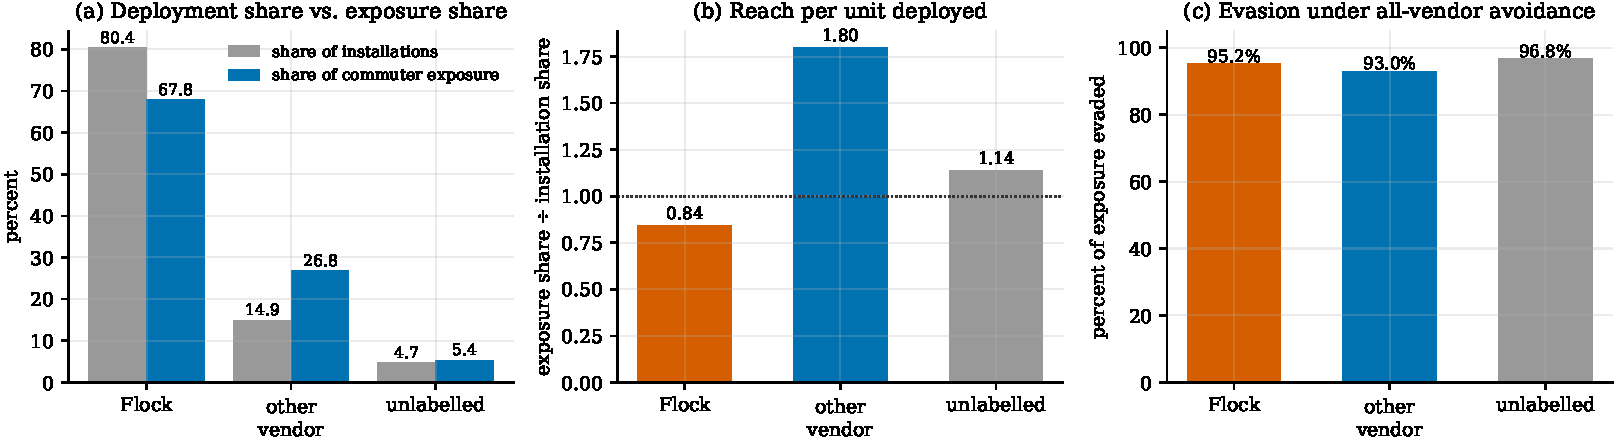
\includegraphics[width=\linewidth]{figures/fig_vendor.pdf}
\caption{Vendor-resolved exposure. (a) Flock's share of exposure falls well below its share
of installations. (b) Per unit deployed, non-Flock cameras reach far more commuters. (c)
Both are avoided at comparable rates under the all-vendor model.}
\label{fig:vendor}
\end{figure}

\begin{table}[t]
\centering
\small
\caption{Vendor-resolved exposure over all \num{17580} routes (\num{98898} camera
encounters). Installation shares are of the \num{140043} cameras that contribute cones,
so they differ slightly from the \num{142991}-node denominator of \Cref{tab:tags}. Flock
holds four-fifths of installations and supplies two-thirds of exposure; per unit deployed,
non-Flock cameras reach \num{2.3}$\times$ as many commuters.}
\label{tab:vendorexp}
\begin{tabular}{lrrrrr}
\toprule
Set & Installations & Exposures & Exposures/\num{1000} cameras & Routes $\geq$1 & Evaded \\
\midrule
Flock Safety  & \SI{81.1}{\percent} & \SI{66.5}{\percent} & \num{585}  & \SI{68.7}{\percent} & \SI{94.8}{\percent} \\
Other vendor  & \SI{14.6}{\percent} & \SI{27.7}{\percent} & \textbf{\num{1356}} & \SI{33.9}{\percent} & \SI{93.2}{\percent} \\
No vendor tag & \SI{4.3}{\percent}  & \SI{5.8}{\percent}  & \num{964}  & \SI{12.6}{\percent} & \SI{96.9}{\percent} \\
\bottomrule
\end{tabular}
\end{table}

Flock Safety holds \SI{81.1}{\percent} of mapped installations but supplies only
\SI{66.5}{\percent} of measured commute exposure. Per unit deployed, non-Flock cameras
generate \textbf{\num{2.3}$\times$} more exposure (\Cref{tab:vendorexp}). The mechanism
is visible in the cone geometry of \Cref{tab:vendorsets}: non-Flock units are multi-head
more than six times as often, and DOT and tolling installations sit on the limited-access
corridors commuters actually use, while a Flock unit watches one residential approach that
fewer commutes cross.

This reframes the vendor's dominance. Flock wins on count and loses on reach: its
deployment model puts many cameras where comparatively few commuters pass, consistent with
a product sold to municipalities and homeowners' associations for neighbourhood coverage
rather than to transport agencies for corridor coverage.

\subsubsection*{The gradient is stronger in transport infrastructure}

Splitting \Cref{sec:results:demo} by vendor locates where the national disparity lives.

\begin{table}[h]
\centering
\small
\caption{Racial composition contrast (\% non-Hispanic Black, Q4/Q1) resolved by vendor and
then subjected to the within-county control of \Cref{sec:results:coverage}.}
\label{tab:vendordemo}
\begin{tabular}{lccl}
\toprule
Camera set & National & Within-county & National verdict \\
\midrule
Flock Safety  & \num{1.28} & \num{0.98} & CIs disjoint \\
Other vendor  & \textbf{\num{1.62}} & \textbf{\num{1.20}} & \textbf{CIs disjoint, both} \\
No vendor tag & \num{1.07} & \num{1.03} & indistinguishable \\
\midrule
All vendors   & \num{1.36} & \num{1.05} & CIs disjoint \\
\bottomrule
\end{tabular}
\end{table}

Both major camera populations show a statistically distinguishable national gradient, but
they are not equal: transport-agency and tolling cameras reach commuters from the highest
quartile of Black population at \num{1.62}$\times$ the rate of the lowest, against
\num{1.28}$\times$ for Flock. The disparity is roughly a quarter larger in infrastructure
that no municipal council votes on.

A historical reading suggests itself. Mid-century urban highway construction routed
limited-access corridors through Black neighbourhoods on a scale that is extensively
documented, and tolling and DOT camera infrastructure sits on exactly those corridors. On
that account the stronger gradient would be a decades-old artefact of road building rather
than a contemporary artefact of camera procurement. We note the hypothesis; this design
cannot test it.

And the discipline of \Cref{sec:results:coverage} applies here, with one exception the
July snapshot did not show. Under within-county ranking Flock's gradient vanishes
(\num{0.98}$\times$) and so does the untagged set's (\num{1.03}$\times$), both with
overlapping intervals. The transport-agency gradient narrows from \num{1.62}$\times$ to
\num{1.20}$\times$---and stays distinguishable, with intervals of \num{1.52}--\num{1.79}
against \num{1.82}--\num{2.15}. It is the only demographic contrast in this paper that
survives the control, and it survives narrowly: two months earlier, on \SI{18}{\percent}
fewer mapped cameras, the same contrast stood at \num{1.18}$\times$ with overlapping
intervals. We report it as what it is: a within-county gradient in tolling and DOT
exposure that is small, present in the September data, and consistent with the corridor
reading above, since a limited-access highway routed through a Black neighbourhood is an
intra-county pattern in a way that a municipality's purchasing decision is not. Holding
RQ5 to a weaker evidentiary standard than RQ3 would have let a between-county artefact
return wearing a vendor label; holding it to the same standard is what lets this one
through.

\paragraph{A correction, and what it cost.}
An earlier pass of this analysis ran on \num{15043} of the \num{17580} routes and reported
that Flock exposure showed \emph{no} racial gradient at all ($\num{0.98}\times$,
overlapping; the July snapshot's full-sample value was $\num{1.20}\times$, disjoint).
That was wrong, and the error is instructive. The route-geometry sidecar is
a gzip file appended to by more than one process, which makes it several concatenated gzip
members; the reader used a single decompressor, which stops at the end of the first member
and returns \emph{successfully}. The missing \SI{14}{\percent} was not merely noise---it
moved Flock from ``no gradient'' to a disjoint gradient and would have supported
a considerably stronger and more quotable claim than the data sustain. We record it
because a silent truncation that returns success is the failure mode least likely to be
caught by inspection, and because the corrected finding is the less convenient one.

\subsection{Two months later: the same commutes against a fifth more cameras}
\label{sec:results:refresh}

Between the two snapshots---2026-07-24 and 2026-09-22---the mapped network grew from
\num{120838} to \num{142991} nodes, \SI{18.3}{\percent}. We re-ran the experiment against
the September cones on the identical \num{17904}-commute sample and the identical road
extract. The same \num{17580} commutes routed (the same 324 did not), and every unavoided
route was identical to the metre and the second, so the comparison is paired and
everything that differs is camera data. Every other number in this paper is from the
September run; this section is what changed.

\begin{table}[t]
\centering
\small
\caption{The same \num{17580} commutes against the two snapshots. Encounters grew by
exactly the growth in mapped cameras; the marginal price of evading one did not move.}
\label{tab:refresh}
\begin{tabular}{lrr}
\toprule
& 2026-07-24 & 2026-09-22 \\
\midrule
Mapped cameras / cone parts        & \num{120838} / \num{114172} & \num{142991} / \num{135210} \\
Camera encounters, all routes      & \num{83565} & \num{98898} (\SI{+18.3}{\percent}) \\
Commutes passing $\geq$1 / $\geq$5 / $\geq$10 & \SI{74.8}{\percent} / \SI{34.6}{\percent} / \SI{14.6}{\percent} & \SI{78.7}{\percent} / \SI{39.7}{\percent} / \SI{18.3}{\percent} \\
Cameras passed, median / mean      & 3 / 4.75 & 3 / 5.63 \\
\nth{90} / \nth{99} percentile     & 12 / 31 & 14 / 35 \\
Exposure rate (cameras/\si{\kilo\metre}) & \num{0.089} & \num{0.105} \\
\midrule
Reduced to zero                    & \SI{84.6}{\percent} & \SI{82.1}{\percent} \\
Extra time, median                 & \SI{1.50}{\minute} & \SI{1.98}{\minute} \\
Avoidance overhead, median         & \SI{5.96}{\percent} & \SI{7.90}{\percent} \\
Minutes per camera evaded, median  & 0.78 & 0.78 \\
\bottomrule
\end{tabular}
\end{table}

Paired, the mean change is \num{+0.87} cameras per commute (\SI{95}{\percent} CI
\num{0.84}--\num{0.91}). \SI{35.5}{\percent} of commutes became more exposed,
\SI{59.7}{\percent} were unchanged, and \SI{4.8}{\percent} became \emph{less} exposed as
cameras were retagged or removed; \num{830} commutes (\SI{4.7}{\percent}) that passed no
camera in July pass at least one in September, and \num{133} went the other way. The
zero-exposure set kept \num{14251} commutes, lost \num{630} and gained \num{179}. The
paired change in avoidance cost is \num{+0.95}~minutes on average (CI \num{0.88}--\num{1.02}),
and a median of zero: most commutes pay exactly what they paid before.

Three things follow.

\textbf{Measured exposure is linear in mapping effort.} Encounters grew by
\SI{18.3}{\percent} against \SI{18.3}{\percent} more mapped cameras. The new cameras were
neither preferentially on commute routes nor preferentially off them, which is what one
expects when the additions are contributors filling in coverage rather than a vendor
targeting corridors. It also says plainly what \Cref{sec:coverage} argues: the absolute
exposure figures are a lower bound that rises with the map, and will keep rising.

\textbf{Refusal got dearer because there is more to refuse, not because each camera is
harder to evade.} The median cost rose by half a minute and the overhead by two points,
while the median price per camera evaded stayed at \SI{0.78}{\minute} to the second
decimal. The road network's capacity to route around a camera did not change; the count
of cameras did. Four commuters in five still reach zero exposure for under two minutes.

\textbf{The states that grew most are the ones we flagged as under-mapped.} Pennsylvania's
mean exposure rose \SI{88}{\percent}, its share of commutes passing any camera from
\SI{40.6}{\percent} to \SI{60.2}{\percent}; Virginia rose \SI{56}{\percent}, North
Carolina \SI{29}{\percent}, Texas \SI{24}{\percent}. Georgia, Illinois, New York and
California---already densely mapped in July---rose \SI{9}{\percent} to
\SI{15}{\percent}. Two months earlier, \Cref{sec:results:coverage} could not distinguish
``Pennsylvania has few cameras'' from ``Pennsylvania has few mappers''. The map now
answers, at least in part: the low-density states were the under-mapped ones, and a
state's July ranking said as much about its contributors as about its cameras. That is
the within-dataset evidence for treating every cross-sectional demographic contrast in
crowdsourced surveillance data as provisional.

\section{Discussion}
\label{sec:discussion}

\subsection{Refusal is cheap, and that is the policy-relevant fact}

The strongest result here is also the simplest: for \SI{82.1}{\percent} of American
commuters, complete avoidance of licence-plate surveillance costs a median of
\SI{1.98}{\minute}. Arguments for \alpr deployment often rest implicitly on ubiquity---the
idea that the network is comprehensive enough that avoidance is futile and therefore the
privacy loss is unavoidable rather than chosen. At current mapped density that premise is
false for four commuters in five---and two months of additional mapping moved that from
five in six without touching the marginal price of a detour.

The corollary cuts the other way. If avoidance is this cheap, it is also cheap for people
with reason to evade legitimate investigation, which bounds how much investigative value a
fixed-camera network can deliver against a motivated subject while it continues to read
every unmotivated one.

\subsection{The equity question is not answerable from crowdsourced data}

We set out to measure whether surveillance burden falls unevenly, and we can report only
that the question is harder than it appears. The national gradient is real in the data,
substantial (\num{1.36}$\times$), and statistically clean---and it evaporates under a
control that any careful reviewer would demand, in every camera population but one, where
a much smaller gradient remains.

We think this generalises. A considerable amount of accessible research on surveillance
infrastructure necessarily rests on volunteer-mapped data, because no authoritative
national inventory exists. Any such study that reports a demographic correlation without
a within-locality control is at serious risk of reporting the demography of \emph{mappers}
rather than of the surveilled. We would encourage that control to become routine.

\subsection{Attention and exposure are aimed at different infrastructure}

Flock Safety is the name in municipal council debates, in local journalism, and in the
activist mapping effort that produced the data underlying this paper. It holds four-fifths
of mapped installations. Yet per unit deployed its cameras reach fewer than half as many
commuters as a tolling or transport-agency camera, and the racial gradient in its exposure
is roughly a quarter weaker.

We do not read this as exonerating, for a reason the measurement itself makes clear. A
camera at the entrance of a residential subdivision does something qualitatively different
from a camera on a toll gantry: it observes a small population repeatedly rather than a
large population once, and repeated observation of a known small set is precisely what
makes pattern-of-life inference possible. Commute exposure measures breadth, not depth, and
Flock's model appears optimised for depth. A study designed around repeat observation of
the same vehicle would likely reverse the ordering reported here, and we would expect it
to.

What the result does establish is that a distributional concern has been attached
disproportionately to one vendor. The infrastructure with the steeper measured gradient is
installed by transport agencies, largely absent from the municipal debate, and sited on
corridors laid down decades before \alpr existed---and it is the one gradient that
persists once tracts are compared only with their neighbours. Regulation aimed only at the vendor
currently in the news would leave the larger measured disparity untouched.

\subsection{Where the burden actually concentrates}

The one distributional finding that does survive is geographic rather than demographic,
and it is counter-intuitive: avoidance is cheapest in dense metropolitan grids and
expensive in rural and intercity travel. Network topology, not camera count, sets the
price of refusal. This is robust to the coverage critique in a way the demographic results
are not, because it depends on road-network structure---which OSM maps close to
completely---rather than on camera counts, which it does not.

\section{Limitations}
\label{sec:limitations}

\subsection{Tract centroids are not addresses}

Every route runs centroid to centroid; real commutes begin in a driveway. In large or
irregular tracts the centroid can sit far from any residence. This adds noise in both
directions and is the main reason we report distributions rather than point estimates.

The stricter caution: tract demographics describe tracts, not the people routed.
``Commutes originating in high-poverty tracts pass more cameras'' is supportable; ``poor
people pass more cameras'' is not.

\subsection{Crowdsourced camera data is non-randomly missing}
\label{sec:coverage}

Absolute exposure figures are a \textbf{lower bound}: where contributors are absent,
cameras are absent from the map but present on the pole. The hazard is not undercounting
but its correlation with the variables of interest, quantified in
\Cref{sec:results:coverage}. Every demographic statement in this paper is conditional on
that, and the condition is not a formality.

\subsection{Cone geometry: swept, and one result depends on it}
\label{sec:lim:geom}

The \SI{60}{\metre} radius was chosen by reasoning---a pole set back from the kerb needs a
cone long enough to reach the carriageway it watches---and the \ang{45} default span from
the \SI{82}{\percent} of explicit arcs that span exactly that. Neither was measured. We
therefore swept the radius over $\{30, 45, 60, 90\}\,\si{\metre}$, rebuilding the cone
geometry at each and re-scoring all \num{17580} routes (\Cref{fig:radius}).

\begin{table}[h]
\centering
\small
\caption{Cone-radius sensitivity. Exposure is mildly sensitive to the assumption; the
avoidance result is not, until the radius grows by half.}
\label{tab:radius}
\begin{tabular}{lrrrr}
\toprule
Radius & Mean cameras & vs \SI{60}{\metre} & Avoided routes still clean & Residual \\
\midrule
\SI{30}{\metre} & \num{4.21} & \num{0.75}$\times$ & \SI{85.5}{\percent} & \SI{5.6}{\percent} \\
\SI{45}{\metre} & \num{5.09} & \num{0.90}$\times$ & \SI{83.6}{\percent} & \SI{5.4}{\percent} \\
\SI{60}{\metre} & \num{5.62} & assumed            & \SI{81.6}{\percent} & \SI{5.6}{\percent} \\
\SI{90}{\metre} & \num{6.29} & \num{1.12}$\times$ & \textbf{\SI{52.4}{\percent}} & \SI{21.0}{\percent} \\
\bottomrule
\end{tabular}
\end{table}

\begin{figure}[t]
\centering
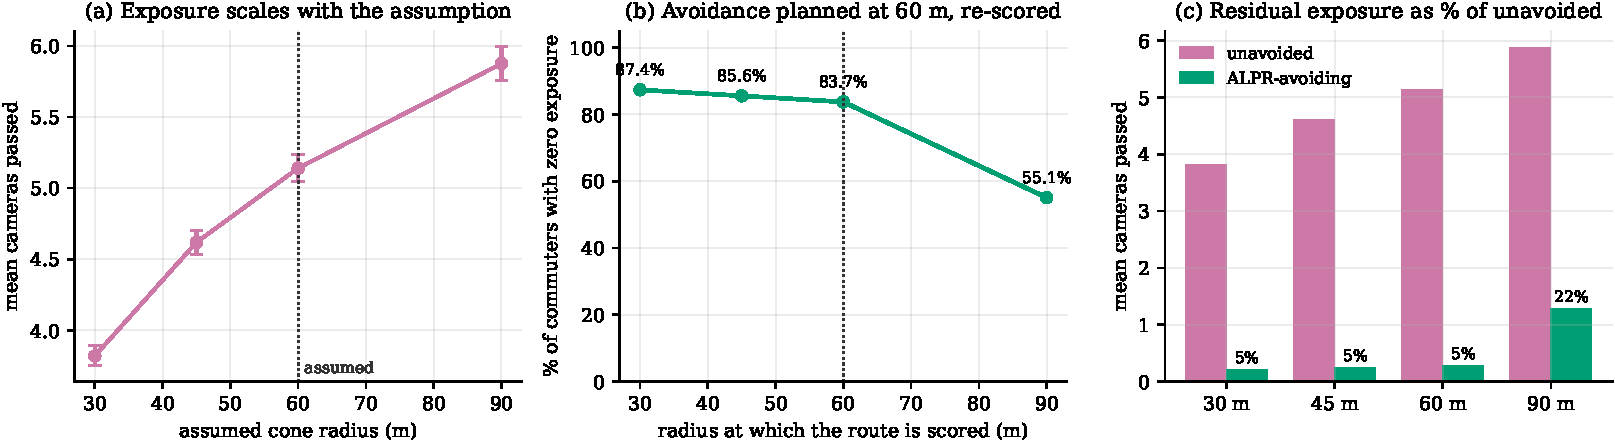
\includegraphics[width=\linewidth]{figures/fig_radius.pdf}
\caption{Sensitivity to the assumed cone radius. (a) Measured exposure scales gently---
halving the radius removes only a quarter of it. (b) The share of commutes reaching zero
exposure is flat below the assumed value and falls sharply above it. (c) Residual exposure
as a fraction of unavoided, by radius.}
\label{fig:radius}
\end{figure}

Two things follow, and they point in opposite directions.

\textbf{Exposure is robust.} Halving the radius removes only a quarter of the measured
exposure, and \SI{90}{\metre} adds \SI{12}{\percent}. Cones are small relative to the road
network at any of these values, so \Cref{sec:results:exposure} does not rest on the choice.

\textbf{The avoidance headline does depend on it.} Routes planned against \SI{60}{\metre}
cones remain clean when re-scored at \SI{45}{\metre} and \SI{30}{\metre}---avoidance is not
finely tuned to the assumption from below. But at \SI{90}{\metre} the share reaching zero
falls from \SI{81.6}{\percent} to \SI{52.4}{\percent}, a drop of \num{29.2} points
(\SI{95}{\percent} CI $[-29.9, -28.6]$), and residual exposure quadruples from
\SI{5.6}{\percent} to \SI{21.0}{\percent} of baseline. If real fields of view are half again
as long as we assume, more than a third of the routes this paper counts as clean are not.

That figure is nonetheless a \emph{lower} bound rather than an estimate, for a reason worth
being precise about. These routes were \emph{planned} against \SI{60}{\metre} cones and only
\emph{re-scored} at \SI{90}{\metre}; a router given \SI{90}{\metre} cones would find
different clean routes, and the denser the network the more of them there are. Measuring
the true value requires a fresh graph import and a complete re-route at each radius---about
nine hours apiece---which we have not done. What the sweep establishes is that the
avoidance claim is conditional on the radius in a way the exposure claim is not, and that
the conditionality bites only above the assumed value.

\subsection{A single avoidance strength}

All results use the maximum strength. Intermediate settings are the practically
interesting ones for a shipped application and they behave badly: the usable range is
roughly $0.3\rightarrow0.01$ and the dead zone is \emph{density-dependent}. A setting of
\num{0.3} does nothing in Delaware while avoiding \SI{62.5}{\percent} of cameras in
Atlanta. A single fixed slider-to-multiplier mapping is therefore not viable; the mapping
must adapt to local density. This is an open problem for the application and an unmeasured
dimension of this paper.

\subsection{Sample scope}

Fifteen states, not fifty. Within-state commutes only (\texttt{od\_main}), so cross-border
metropolitan areas---New York/New Jersey, Philadelphia, Washington DC, Kansas City, St
Louis, Portland---are systematically truncated at the state line. Several are exactly the
dense multi-jurisdiction areas where the question is most pointed.

\subsection{Two snapshots, two months apart}

The network is expanding quickly---\SI{18}{\percent} more mapped nodes between 2026-07-24
and 2026-09-22---and absolute figures date accordingly; \Cref{sec:results:refresh} shows
measured exposure rising in proportion to the map. The relative claims held across the two
snapshots: the cheapness of refusal (a marginal \SI{0.78}{\minute} per camera in both), the
metro/rural asymmetry, and the within-county collapse of the pooled gradient. Two months is
a short baseline. The one conclusion that changed between them---the within-county
transport-agency gradient becoming distinguishable---changed in the direction that growing
coverage should move a real but small effect, and also in the direction it would move a
mapping artefact concentrated in a few counties; a third snapshot would separate those.
Routing uses free-flow speeds with no traffic, time-of-day, or turn-restriction penalties,
so both travel times are optimistic. The \emph{difference} between them---the quantity
actually reported---is more robust than either absolute, since both share the bias.

\subsection{Avoidance is a preference, not a guarantee}

\texttt{multiply\_by: 0.01} makes observed roads expensive, not impassable. Where no
alternative exists the router correctly uses the watched road. ``Zero cameras'' means the
optimiser found a clean path, not that one was guaranteed to exist.

\section{Reproducibility}

Fixed seed \texttt{20260725} throughout, for both sampling and bootstrap. All external
data sources are public and require no API key.

\begin{table}[h]
\centering
\small
\begin{tabular}{ll}
\toprule
Component & Path \\
\midrule
Data acquisition            & \texttt{research/data/fetch.sh} \\
Camera fetch (continental)  & \texttt{server/alpr/fetch-na-cones.sh} \\
Cone construction           & \texttt{server/alpr/build\_cones.py} \\
Cone-set variants           & \texttt{server/alpr/build-variants.sh} \\
Snapshot statistics         & \texttt{research/scripts/snapshot\_stats.py} \\
Routing configuration       & \texttt{server/graphhopper/config/trames.yml} \\
Graph build                 & \texttt{server/graphhopper/rebuild-with-cones.sh} \\
Commute sampling            & \texttt{research/scripts/build\_sample.py} \\
Experiment                  & \texttt{research/scripts/run\_experiment.py} \\
Geometry backfill           & \texttt{research/scripts/backfill\_geometry.py} \\
Vendor rescoring            & \texttt{research/scripts/vendor\_exposure.py} \\
Analysis                    & \texttt{research/scripts/analyze.py} \\
Post-processing, one command & \texttt{research/scripts/run-analyses.sh} \\
Snapshot comparison         & \texttt{research/scripts/compare\_snapshots.py} \\
Figures                     & \texttt{research/paper/make\_figures.py} \\
\bottomrule
\end{tabular}
\end{table}

\noindent
The \SI{18}{\giga\byte} OSM extract and \SI{14}{\giga\byte} graph cache are not
redistributed; the acquisition and import scripts rebuild both.

\end{document}
